\section{Architecture and design}
\label{sec:Design}

	The design of the program is very simple. In we place ourselves in the context of object-oriented programming (since it is the most understandable form of design by a human), the program is composed of 5 classes (it could even be less than that). Those are depicted in the following UML diagram :

\begin{figure}[H]
\centering
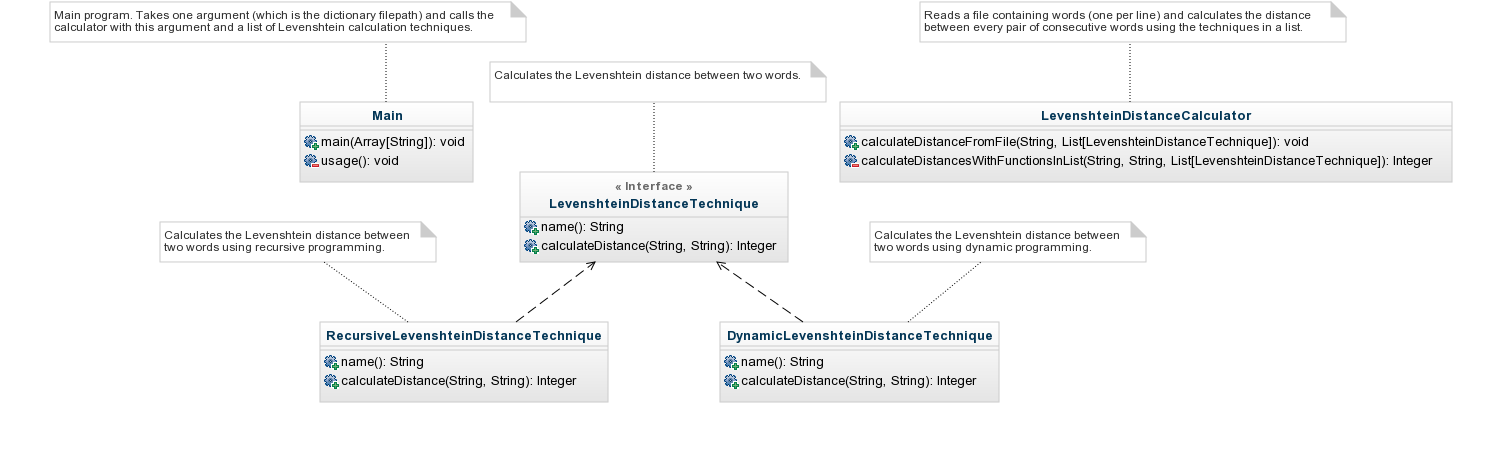
\includegraphics[width=\textwidth]{uml.png}
\caption{UML diagram of the algorithm in Scala}
\label{fig:uml}
\end{figure}